\documentclass[14pt]{beamer}

%encoding
\usepackage[utf8]{inputenc}

%language
\usepackage[english, russian]{babel}
\usepackage{amsmath}
\usepackage{bm}
\usepackage{graphicx}
\usepackage{hyperref}
\usepackage{setspace}
\usepackage{tikz}
\usepackage{adjustbox}
\usepackage{marvosym}
\usepackage{animate}
\usetikzlibrary{shapes,arrows,positioning}
\makeatletter
\makeatother
\graphicspath{{images/}}

\usepackage{tikz}
\usetikzlibrary{shapes,arrows}

\tikzstyle{decision} = [diamond, draw, fill=blue!20, text width=4.5em, text badly centered, node distance=3cm, inner sep=0pt]
\tikzstyle{block} = [rectangle, draw, fill=blue!20, text width=11em, text centered, rounded corners, minimum height=2em]
\tikzstyle{line} = [draw, -latex    ]
\tikzstyle{cloud} = [draw, ellipse,fill=red!20, node distance=3cm, minimum height=2em]

\setbeamerfont{author in head/foot}{size=\small}
\setbeamerfont{title in head/foot}{size=\footnotesize}
\setbeamercovered{invisible}
\setbeamertemplate{navigation symbols}{}%remove navigation symbols

\title[Modeling of heart valve]{Mathematical modelling of artificial heart valve performance}
\date{\today}
\author[D.A. Dolgov]{D.A. Dolgov, Y.N. Zakharov}
\institute{
    Kemerovo State University\\
    \vspace{0.7cm}
    \vspace{0.7cm}
}
\usetheme[numbers, totalnumbers, minimal, nologo]{Statmod}
\usefonttheme[onlymath]{serif}

\definecolor{statmodblue}{RGB}{100,10,30}
\definecolor{statmodsand}{RGB}{244,215,103}

\begin{document}
\begin{otherlanguage}{english}
\maketitle
\end{otherlanguage}

%description of the problem
\begin{frame}
\frametitle{Introduction}
Artificial heart valves are an effective method to treat many cardiovascular
diseases. They are one of the most sophisticated medical devices that are used
in cardiac surgery because of their design features. There are many
requirements to the functioning of the artificial heart valves - an ideal valve
replacement should produce a low flow resistance, yield a small regurgitant
volume, minimise turbulence, etc.
\end{frame}
\note{
    объем регургитации - объем обратного течения (из желудочка в атриум)

    Каждый год в мире
    проводится примерно 250 000 операций по восстановлению или замене
    поврежденных сердечных клапанов, и наблюдается тенденция к росту этого
    числа - Institute D.C.R. {\em Adult cardiac surgery database, executive summary} \url{http://www.sts.org/sites/default/files/documents/2015Harvest2_ExecutiveSummary.pdf}, 2015.

}

\begin{frame}
\frametitle{Research overview}
    There are many researches, in which valves are of primary interest, while ignoring the fluid-structure interaction.
    \par
    {\tiny
        \begin{itemize}
            \item[\MVRightarrow] Bockeria L. A., Skopin I. I., Sazonenkov M. A., Tumaev E. N. Stress in valve leaflets and bioprosthesis in mitral position. Influence of fibrous ring on leaflet stress. // Clinical physiology of blood circulation, 2008, №2
            \item[\MVRightarrow] Kunzelman K.S., Reimink M.S. et al  Annular dilatation increases stress in the mitral valve and delays coaptation: a finite element computer model. (1997) Cardiovasc Surg 5(4):427–434
            \item[\MVRightarrow] Weinberg E. Dynamic simulation of heart mitral valve with transversely isotropic material model. Massachusetts Institute of Technology (2005)
            \item[\MVRightarrow] Kim H.S. Nonlinear multi-scale anisotropic material and structural models for prosthetic and native aortic heart valves. Georgia Institute of Technology (2009)
        \end{itemize}
    }
\end{frame}
\note{
    Отметить, что рассматриваются работы, посвященные именно математическому моделированию клапанов,
    а не экспериментальному. На эту тему мало русскоязычных работ - даже в монографии "Искусственные клапаны сердца"
    (Орловский, Гриценко, Юхнев, Евдокимов, Гавриленков),
    где описан крупный вклад отечественных ученых в области клапанов, в разделе "Математическое моделирование" нет
    упоминаний о русскоязычных работах.
    Существует достаточно много (по крайней мере, зарубежных) исследований,
    посвященных математическому моделированию сердечных клапанов. В ранних моделируются
    только достаточно простые клапаны (по структуре, двумерные и проч.).
    Существует много современных работ, которые изучают клапан только с точки зрения
    эластичности, напряжений, возникающих при деформации и проч (при этом данные о давлении жидкости
    берутся либо из эксперимента, либо упрощенные, например течение Пуазеля).
    Самый перспективный вид исследований те, которые полноценно описывают взаимодействие потока и клапана,
    т.е. IBM
}

\begin{frame}
\frametitle{Research overview}
    Most of the researches, which considering full fluid-structure interaction,
    are related to the immersed boundary method. But in the existing papers the fluid flow
    with admixtures is covered not enough.
    \par
    {\tiny
        \begin{itemize}
            \item[\MVRightarrow] Peskin, Charles S. "Numerical analysis of blood flow in the heart." Journal of computational physics 25.3 (1977): 220-252.
            \item[\MVRightarrow] Luo, X. Y., et al. "Effect of bending rigidity in a dynamic model of a polyurethane prosthetic mitral valve." Biomechanics and modeling in mechanobiology 11.6 (2012): 815-827.
            \item[\MVRightarrow] Flamini, Vittoria, Abe DeAnda, and Boyce E. Griffith. "Immersed boundary-finite element model of fluid-structure interaction in the aortic root." (2015).
        \end{itemize}
    }
\end{frame}

% valves placement
\begin{frame}
\frametitle{Arrangement of the valves}
    \begin{center}
        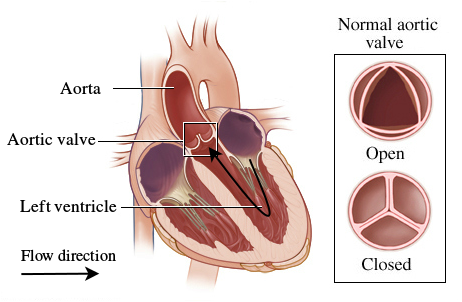
\includegraphics[width=8.5cm]{aorta_scheme.png}
    \end{center}
\end{frame}

\begin{frame}
\frametitle{Example of artificial heart valve}
    \begin{center}
        \vspace{1.0cm}
        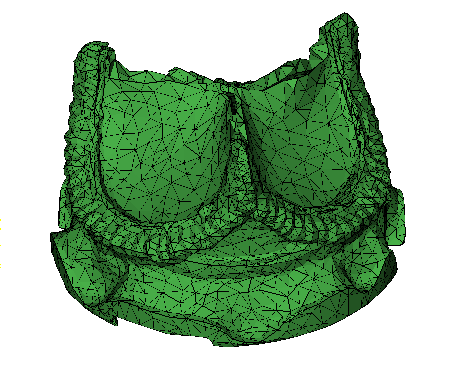
\includegraphics[width=6cm]{real_valve_3_1.png}
        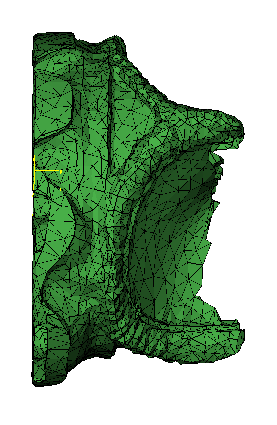
\includegraphics[width=3cm]{real_valve2_1.png}

        \vspace{1.1cm}
        \mbox{\scriptsize
            <<Uniline>>, ФГБУ НИИ КПССЗ СО РАМН, г. Кемерово
        }
    \end{center}
\end{frame}

% valve tissue structure
\begin{frame}
\frametitle{Scheme of valve tissue structure}
    \begin{center}
        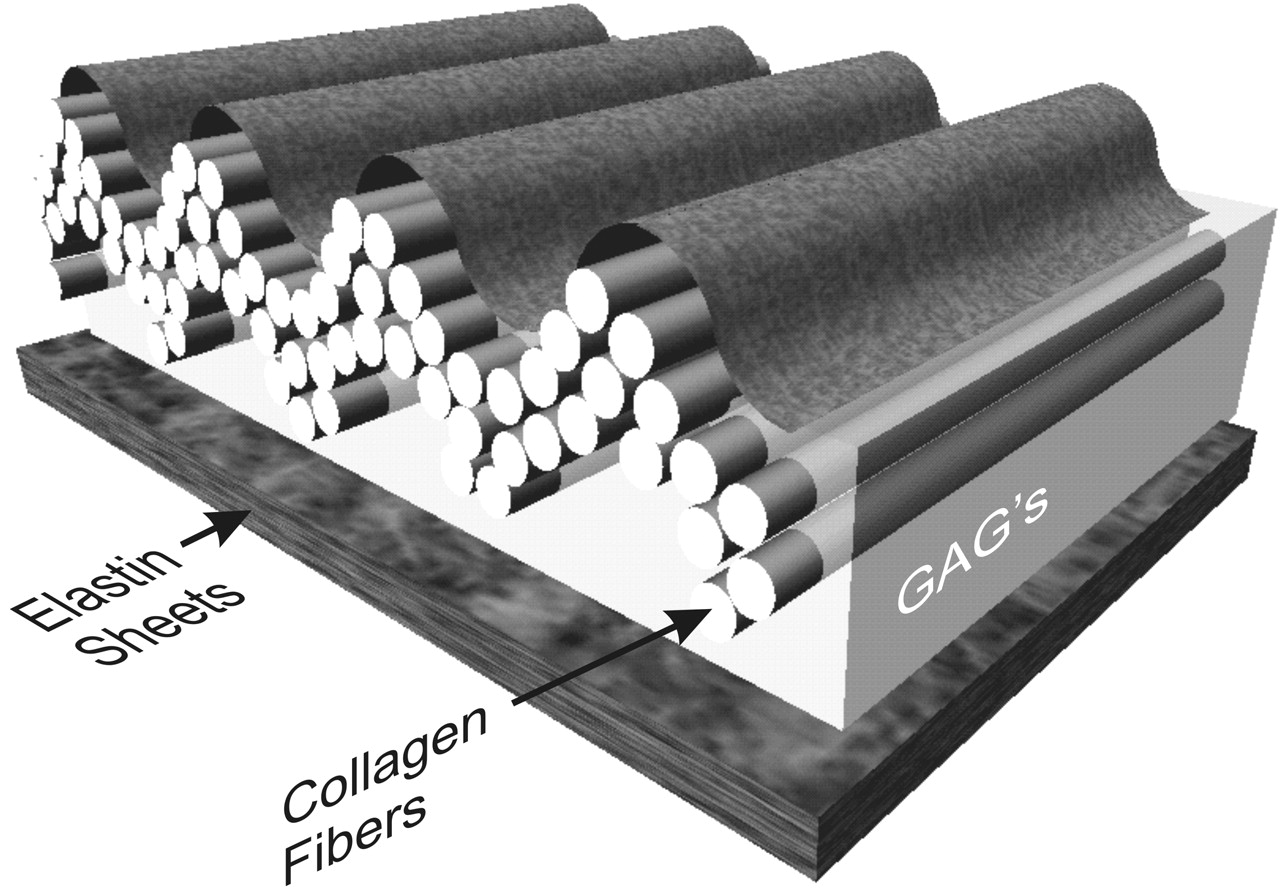
\includegraphics[width=8.5cm]{valve_tissue_structure.jpg}
    \end{center}

    \begin{spacing}{0.5}
        \mbox{\scriptsize
            Vesely, Ivan. <<Heart valve tissue engineering.>> Circulation research 97.8 (2005): 743-755.
        }
    \end{spacing}

\end{frame}
\note{
    \begin{itemize}
        \item коллагеновые волокна (collagen fibers)
        \item слой эластина (белок) (elastin sheet)
        \item гликозаминогликаны (glycosaminoglycan matrix)
    \end{itemize}
}

% blood structure scheme
\begin{frame}
\frametitle{Scheme of blood structure}
    \begin{center}
        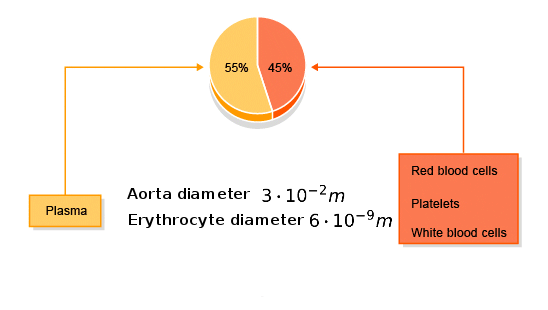
\includegraphics[width=8.5cm]{blood_scheme3.png}
    \end{center}
\end{frame}

\begin{frame}
\frametitle{Model description}
We will consider the problem of blood flow inside large vessels with flexible
walls and valve.  Blood consists of plasma and formed elements. Valve leaflets
are deformed under the fluid pressure.  We model the blood as a viscous
incompressible inhomogeneous two component fluid with variable viscosity, and
vessel wall and valve leaflets as a fluid impermeable surface with specified
stiffness.
\end{frame}

%description of the problem: schema
\begin{frame}
\frametitle{Model description}
    \begin{center}
        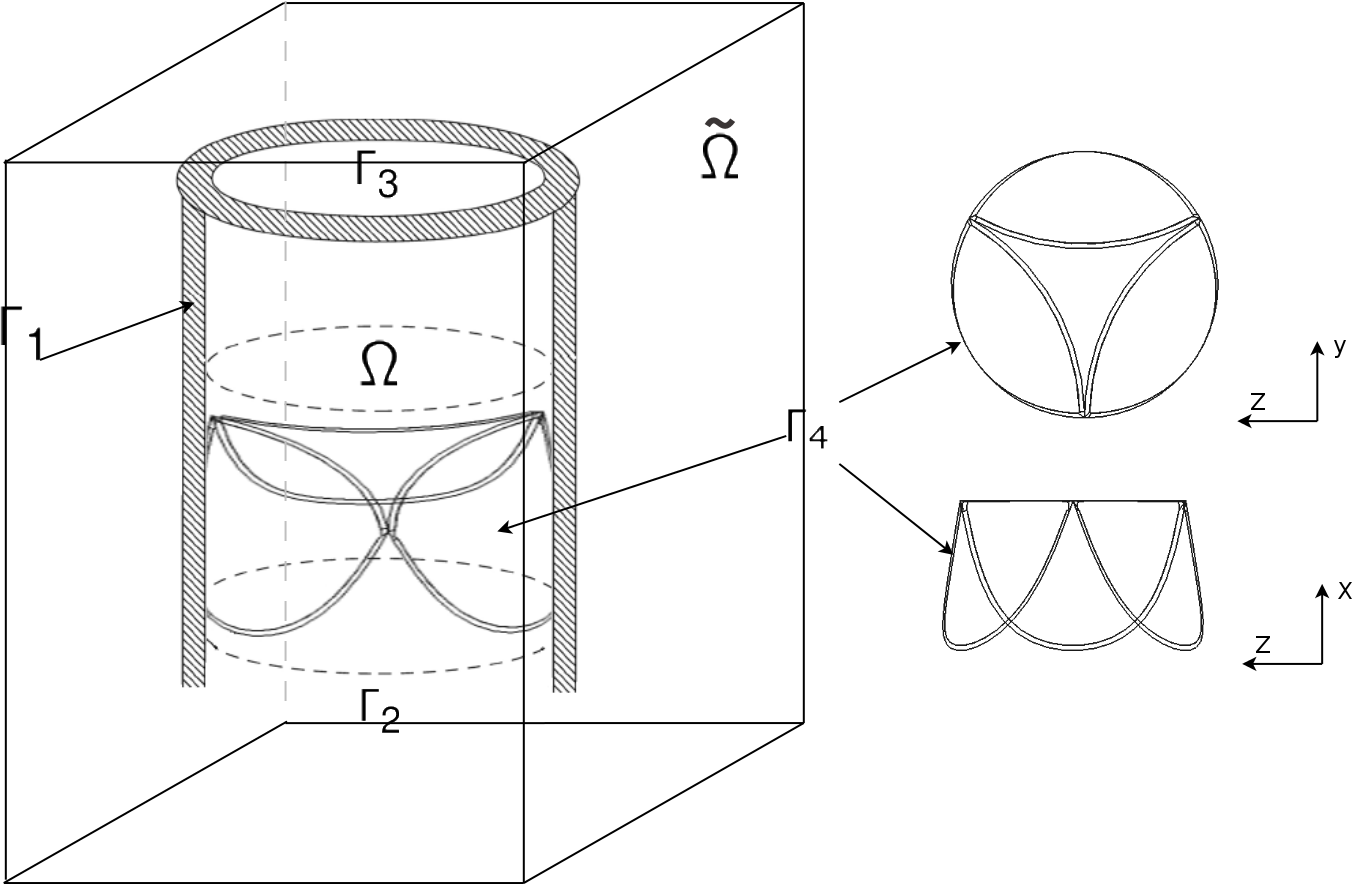
\includegraphics[width=10cm]{aorta_valve_scheme_flat_computation.png}
    \end{center}
\end{frame}
\note{$\Gamma_1$ - гибкие стенки, $\Gamma_2,\Gamma_3$ - вход/выход}

% navier stokes equations
\begin{frame}
\frametitle{Fluid flow}
Navier-Stokes system of equations:
\begin{gather}
    \label{eq:motion}
    \frac{\partial u}{\partial t} + (u \cdot \nabla) u = - \frac{1}{\rho} \nabla p + \nabla \cdot \sigma + f\\
    \label{eq:continuity}
    \frac{\partial \rho}{\partial t} + \nabla \cdot (\rho u) = 0
\end{gather}
where $\sigma = \mu (\nabla u + (\nabla u)^{T})$, $\bar{x} = (x, y, z) \in \Omega$ with the initial and boundary conditions
\begin{gather*}
    u(\bar{x}, t_0) = u_0;\ \frac{\partial u}{\partial n}|_{\Gamma_2, \Gamma_3} = 0\\
    p|_{\Gamma_2} = p_{in};\ p|_{\Gamma_3} = p_{out} \\
\end{gather*}

\end{frame}
\note{Уравнения записаны в векторном виде, $\sigma$ - вязкий тензор напряжений}

% concentration
\begin{frame}
\frametitle{Concentration}
An equation for the concentration of admixture in the fluid:
\begin{gather}
    \label{eq:concentration}
    \frac{\partial c}{\partial t} + u \cdot \nabla c = 0
\end{gather}
with the initial and boundary conditions
\begin{gather*}
    c(\bar{x}, 0) = c_0(\bar{x})\\
    c(\bar{x}, t)|_{\Gamma_2} = c_s(\bar{x}, t)
\end{gather*}

\end{frame}

% concentration: dependencies
\begin{frame}
\frametitle{Concentration}
Density and viscosity are depend from concentration:
\begin{gather}
    \label{eq:concentration_viscosity}
    \mu = c (\mu_2 - \mu_1) + \mu_1\\
    \label{eq:concentration_density}
    \rho = c (\rho_2 - \rho_1) + \rho_1
\end{gather}

where $\mu_1, \mu_2, \rho_1, \rho_2$ - viscosity and density of both components.
\end{frame}

% boundary
\begin{frame}
\frametitle{Deformation resistance}
Motion of the vessel walls and valve leaflets is defined by the forces, which
return them to the original position.
\begin{gather}
    \label{eq:strain_energy}
    F =  \frac{\partial}{\partial s}(T \tau) + \frac{\partial^2}{\partial s^2} \Big( E \cdot I \frac{\partial^2}{\partial s^2} X \Big)
\end{gather}
\begin{gather}
    \label{eq:define_boundary_force}
    F = k \cdot \|X - X_0\|
\end{gather}
\begin{flalign*}
    &E - \mbox{Young's modulus}\\
    &I - \mbox{cross section moment of inertia}\\
    &T - \mbox{fiber tension}\\
    &\tau - \mbox{unit tangent vector}
\end{flalign*}
\end{frame}
\note{$E$ - модуль Юнга, $I$ - момент инерции поперечного сечения, $T$ - напряжение фибры, $\tau$ - единичный тангенциальный вектор, касательный к фибре.}

% solve method:immersed boundary
\begin{frame}
\frametitle{Fluid-structure interaction}
Interaction between valve leaflets and fluid flow:
\begin{gather}
    \label{eq:ibm_velocity}
    \frac{\partial X}{\partial t} = \int_{\Omega_h} u \cdot \delta (\bar{x} - X)\; dx\; dy\; dz \\
    \label{eq:ibm_force}
    f = \int_{\Gamma_h} F \cdot \delta (\bar{x} - X)\; dq\; dr\; ds\\
    \label{eq:no_slip}
    \frac{\partial X}{\partial t} (q, r, s, t) = u(X(q, r, s, t), t)
\end{gather}
\end{frame}
\note{Заглавные символы относятся к погруженной границе, обычные - к жидкости}

% solve method
\begin{frame}
\frametitle{Solution method}
We determine the fluid flow and the valve leaflets on the separate grids
\begin{itemize}
    \item[\MVRightarrow] $\Omega_h = \Omega_h(x, y, z)$ - uniform staggered grid for fluid.
    \item[\MVRightarrow] $\Gamma_h = \Gamma_h(q, r, s, t)$ - grid, related to the valve leavlets with Lagrangian coordinate system.
t\end{itemize}

\end{frame}
\note{При обтекании жидкость какого-либо тела, она испытвает влияние силы давления рядом с границей тела (и сдвиговые силы, если есть условие прилипания). Исходя их этого обтекание тела можно моделировать с помощью поля внешних сил}

% solve method:split scheme
\begin{frame}
\frametitle{Solution algorithm: flow}
Splitting schemes due to physical factors:
\begin{gather}
    \label{eq:split_first}
    \frac{u^* - u^n}{\triangle t} = - (u^n \cdot \nabla) u^n + \frac{1}{\rho} \nabla \sigma + f\\
    \label{eq:split_second}
    \rho \triangle p^{n+1} - (\nabla \rho \cdot \nabla p^{n+1}) = \frac{\rho^2 \nabla u^*}{\triangle t}\\
    \label{eq:split_third}
    \frac{u^{n+1} - u^*}{\triangle t} = - \frac{1}{\rho} \nabla p^{n+1}
\end{gather}
где $\nabla \sigma (u^n, \mu) = \mu \triangle u^n + (\nabla \mu \cdot \nabla) u^n + (\nabla \mu \cdot J_{u^n}) $
\end{frame}
\note{
    \begin{itemize}
        \item[\MVRightarrow] Решаем уравнение \eqref{eq:split_first} методом стабилизирующей поправки (Дугласа-Рекфорда)
        \item[\MVRightarrow] Из уравнения \eqref{eq:split_second} методом бисопряженных градиентов определяем поле давления
        \item[\MVRightarrow] Восстанавливаем окончательное поле вектора скорости по явным формулам \eqref{eq:split_third}
    \end{itemize}
}

% solve method: boundary forces
\begin{frame}
\frametitle{Solution algorithm: valve}
\begin{gather}
    \label{eq:strain_energy}
    F_{n} =  \frac{\partial}{\partial s}(T_{n} \tau_{n}) + \frac{\partial^2}{\partial s^2} \Big( E \cdot I \frac{\partial^2}{\partial s^2} X_{n} \Big)
\end{gather}
\end{frame}
\note{$E$ - модуль Юнга, $I$ - момент инерции поперечного сечения, $T$ - напряжение фибры, $\tau$ - единичный тангенциальный вектор, касательный к фибре.}

% solve method:ibm scheme
\begin{frame}
\frametitle{Fluid-structure interaction}
Interpolation of the flow velocity on the immersed boundary, and new body
forces distribution:
\begin{gather}
    \label{eq:interpolation}
    U_n = \sum_{ijk}u_{ijk} \cdot D(x_{ijk} - x_n) h_{ijk}^3 \\
    \label{eq:spreading}
    f_{ijk} = \sum_n F_n \cdot D(x_{ijk} - x_n) h^2_n
\end{gather}

$D(x_n)$ corresponds to $\delta(x - x_k)$.
\end{frame}

% totals and examples
% use avconv -i video.avi -vsync 1 -r 10 -an -y 'data_%d.png'
% to create series of png for animation

\begin{frame}
\frametitle{<<Uniline>> dynamics}
    %\animategraphics[autoplay,loop,width=\textwidth]{20}{animation/real_valve/data_}{1}{108}
    \animategraphics[autoplay,loop,width=\textwidth]{20}{animation/real_valve/data_}{1}{1}
\end{frame}

\begin{frame}
\frametitle{<<Uniline>> dynamics}
    %\animategraphics[autoplay,loop,width=\textwidth]{20}{animation/uniline_tracks/data_}{1}{108}
    \animategraphics[autoplay,loop,width=\textwidth]{20}{animation/uniline_tracks/data_}{1}{1}
\end{frame}

\begin{frame}
\frametitle{Распределение примеси}
    %\animategraphics[autoplay,loop,width=\textwidth]{20}{animation/valve_in_mixture/data_}{1}{201}
    \animategraphics[autoplay,loop,width=\textwidth]{20}{animation/valve_in_mixture/data_}{1}{1}
\end{frame}

\begin{frame}
\frametitle{Leaflets rotation}
    %\animategraphics[autoplay,loop,width=\textwidth]{20}{animation/rotation/data_}{1}{135}
    \animategraphics[autoplay,loop,width=\textwidth]{20}{animation/rotation/data_}{1}{1}
\end{frame}

\begin{frame}
\frametitle{Stress distribution}
    \begin{center}
        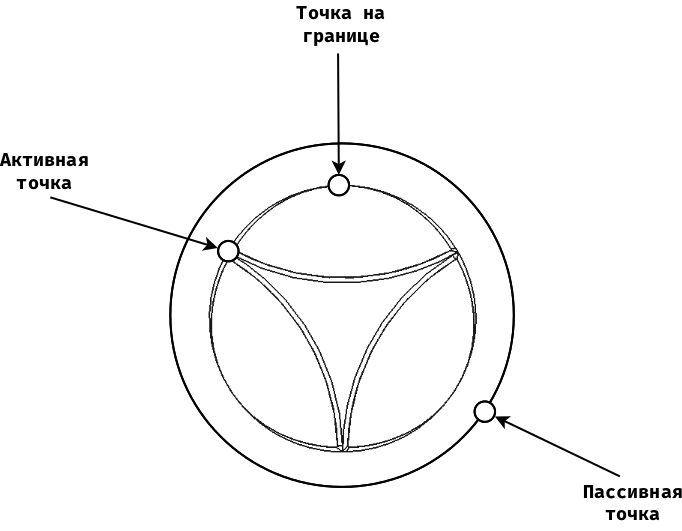
\includegraphics[width=9cm]{valve_points.png}
    \end{center}
\end{frame}

\begin{frame}
\frametitle{Stress distribution}
    \begin{center}
        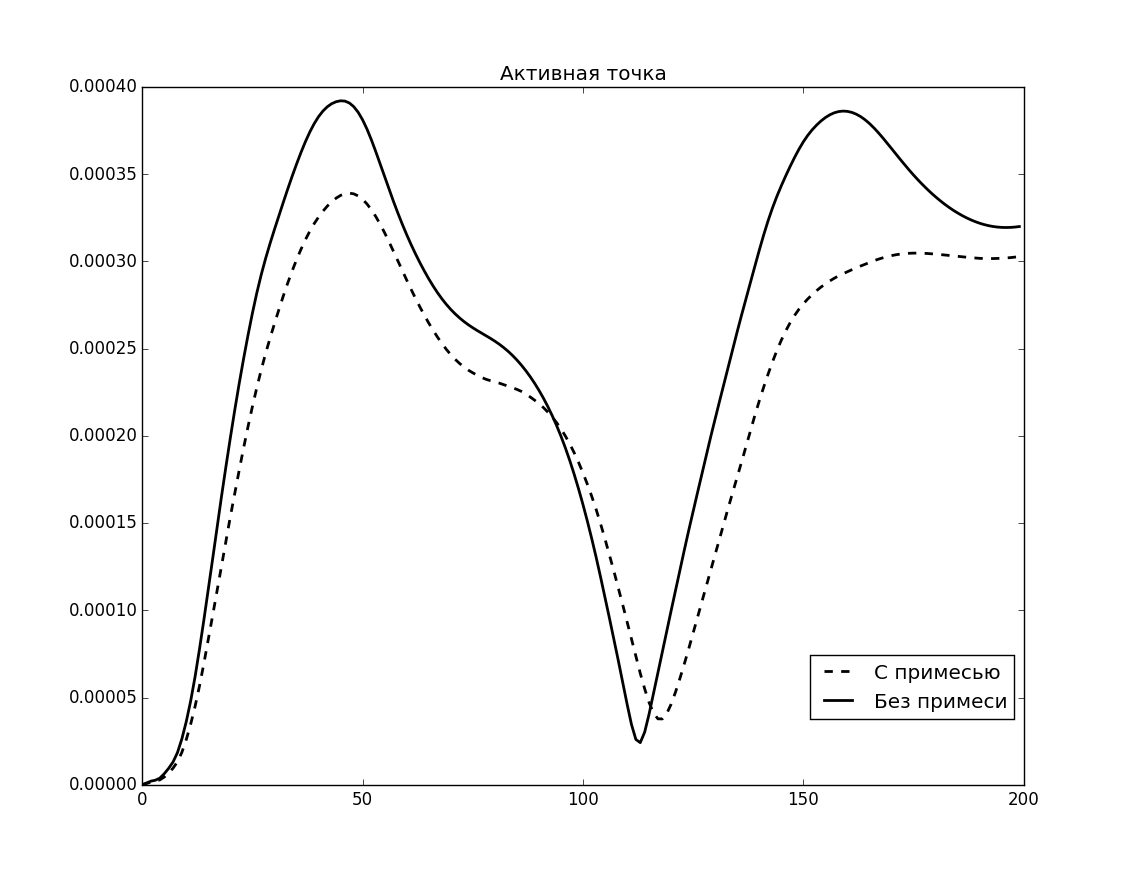
\includegraphics[width=10cm]{forces_active_point.png}
    \end{center}
\end{frame}

\begin{frame}
\frametitle{Stress distribution}
    \begin{center}
        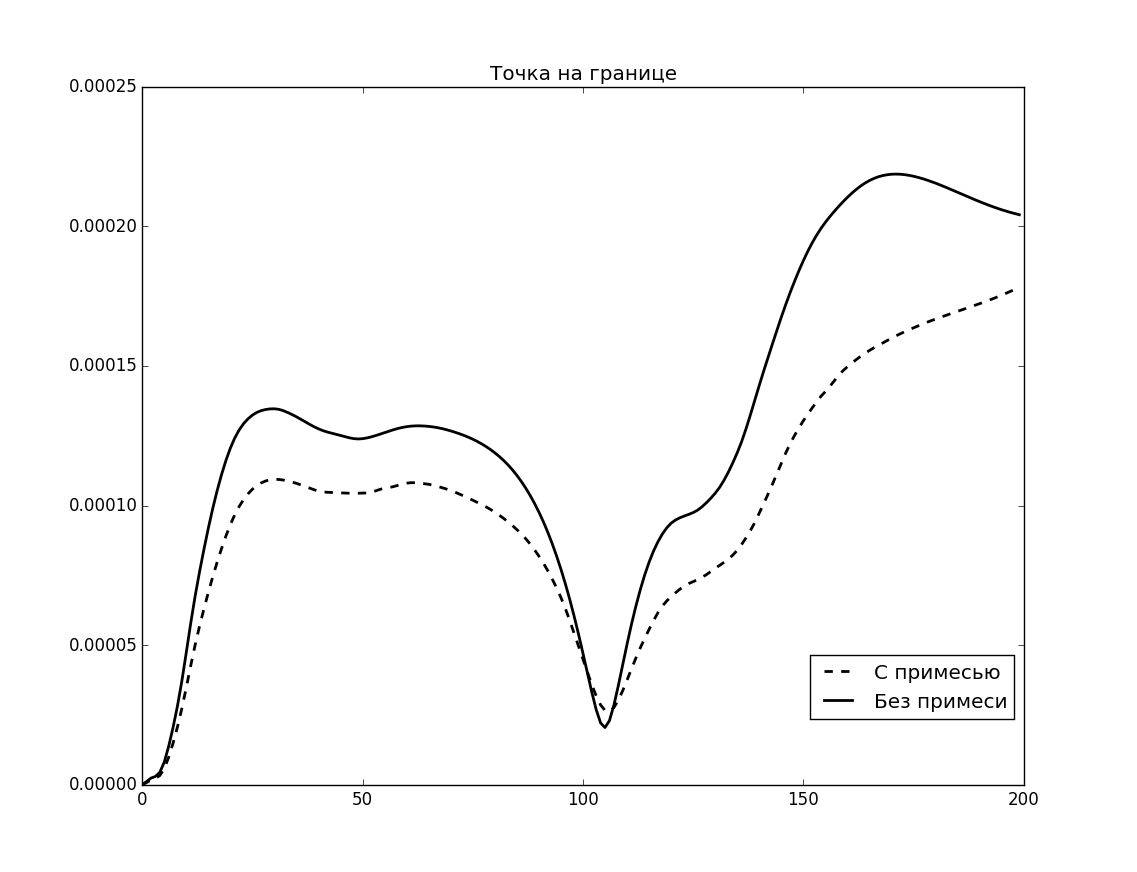
\includegraphics[width=10cm]{forces_boundary_point.png}
    \end{center}
\end{frame}

\begin{frame}
\frametitle{Stress distribution}
    \begin{center}
        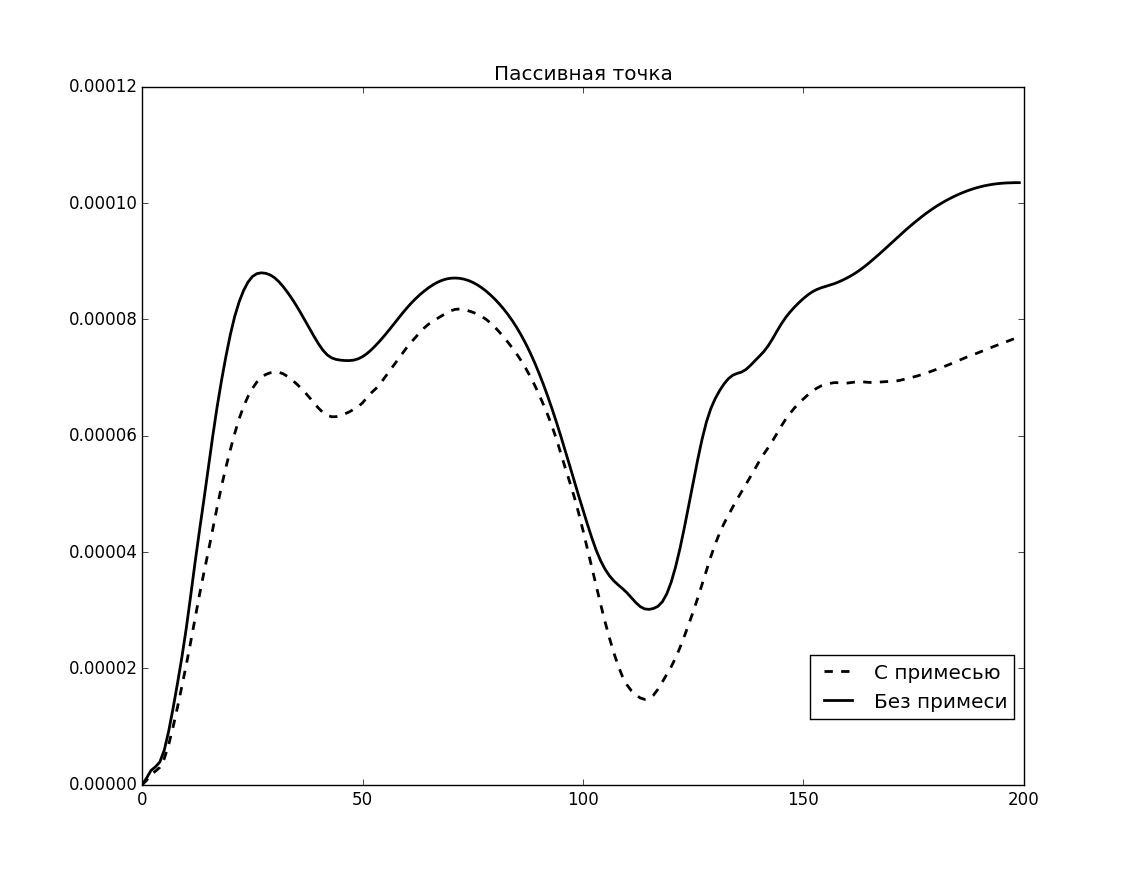
\includegraphics[width=10cm]{forces_passive_point.png}
    \end{center}
\end{frame}

\begin{frame}
\frametitle{Flow rate}
    \begin{center}
        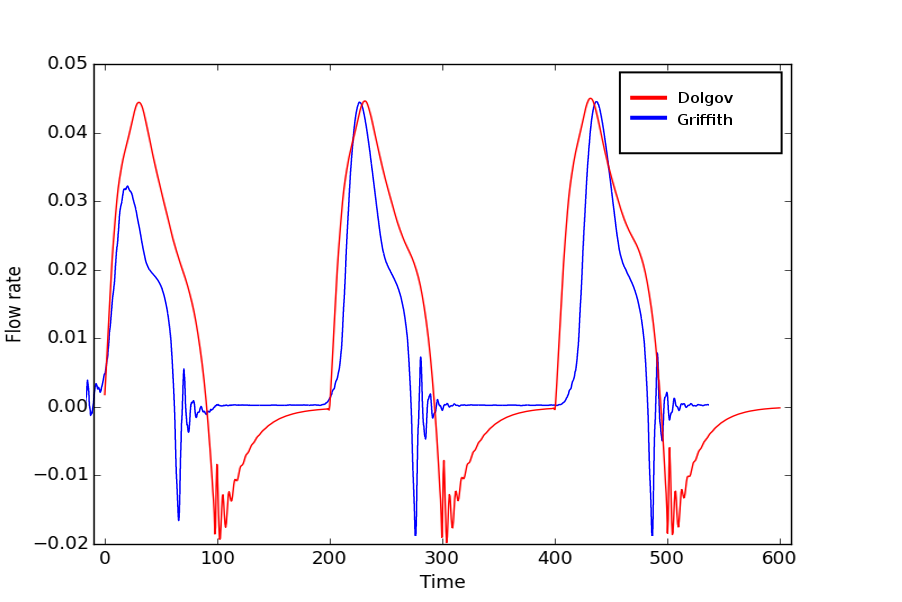
\includegraphics[width=10cm]{flow_rate_comparison_with_legend.png}
    \end{center}
\end{frame}

\begin{frame}
\frametitle{Flow rate}
    \begin{center}
        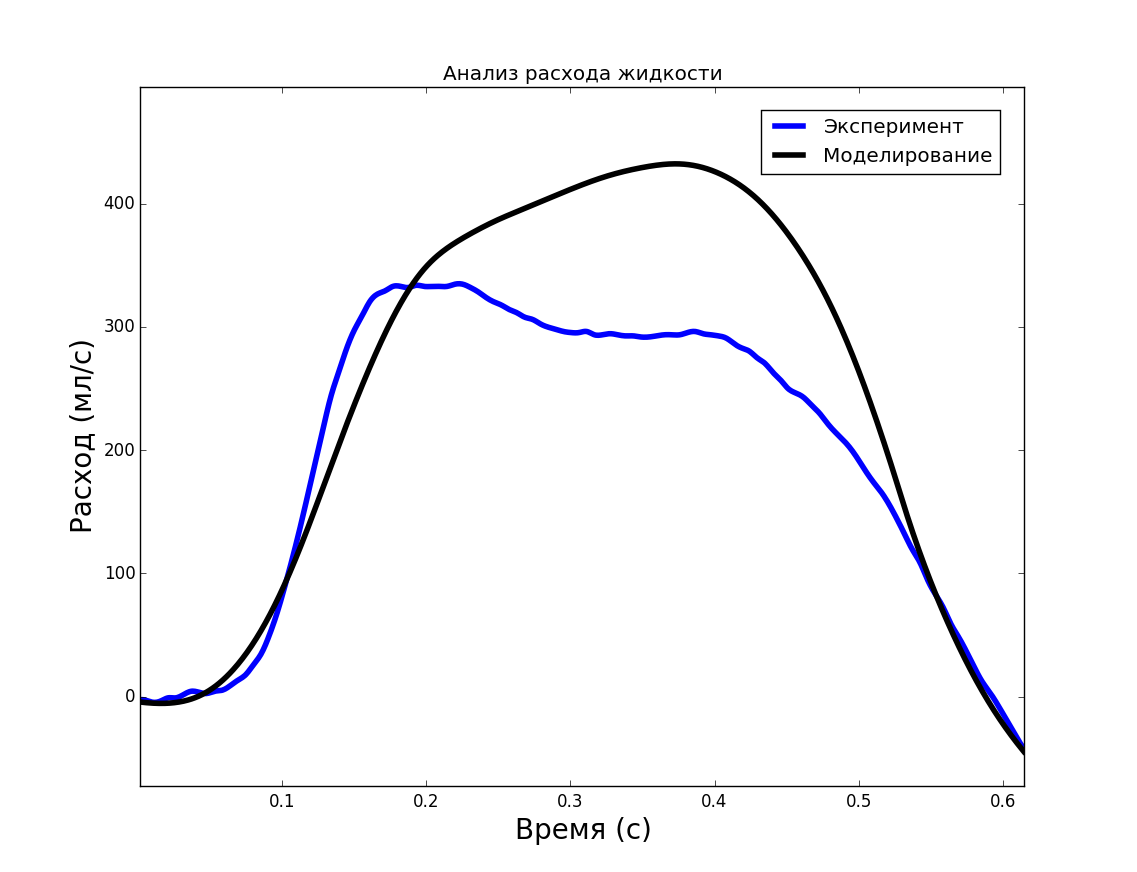
\includegraphics[width=10cm]{flowrate_experiment_with_legend.png}
    \end{center}
\end{frame}

\begin{frame}
\frametitle{Flow rate}
    \begin{center}
        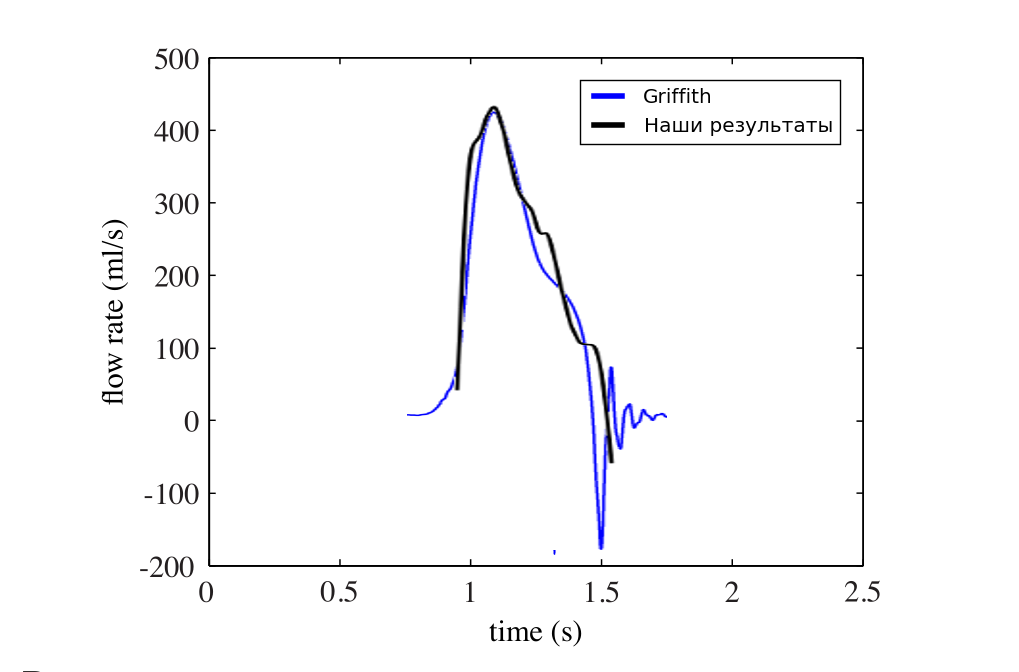
\includegraphics[width=10cm]{flow_rate_griffith_comparison3.png}
    \end{center}
\end{frame}

\end{document}
